\section{Durchführung}
Bevor mit der eigentlichen Messung begonnen werden kann, muss zunächst eine Justage des Versuchsaufbaus
vorgenommen werden. In Abbildung \ref{fig:aufbau} ist der verwendete Versuchsaufbau schematisch 
dargestellt.
\begin{figure}[H]
    \centering
    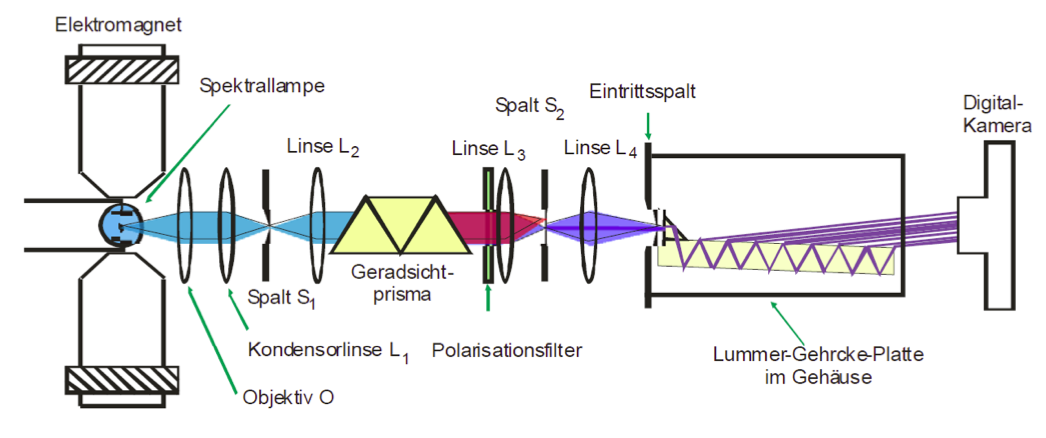
\includegraphics[width=0.8\textwidth]{../images/Aufbau.png}
    \caption{Schematische Darstellung des verwendeteten Versuchsaufbau zur Untersuchung der Zeeman-Effektes \cite{anleitung}.}
    \label{fig:aufbau}
\end{figure} \noindent
Wie in der Abbildung zu erkennen ist befindet sich im Zentrum eines Elektromagneten die Spektrallampe. Das Licht 
wird duch eine Linse auf einen größenverstellbaren Spalt fokussiert. Daraufhin passiert das Licht eine 
weitere Linse bevor es durch ein Geradsichtprisma in seine spektralen Anteile aufgespalten wird. 
Mithilfe einer Kombination aus Linsen und einem weiteren Spalt wird die zu untersuchende Wellenlänge 
auf den Eintrittsspalt der Lummer-Gehrcke-Platte gelenkt. Im Inneren dieser befinden sich parallele Platten 
an denen das Licht reflektiert wird, wobei immer ein geringer Anteil aus dem Glas austritt. 
Dadurch kommt es zu Interferenzerscheinungen, die mithilfe einer Digitalkamera aufgenommen werden.\\
Es ist sicherzustellen, dass die optischen Bauteile so eingestellt sind, dass eine möglichst hohe 
Intensität in die Lummer-Gehrcke-Platte einfällt. \\
Im ersten Schritt der Messungen wird das Magnetfeld geeicht. Dafür wird das Magnetfeld im Inneren 
des Elektromagneten mithilfe einer Hallsonde in Abhängigkeit des angelegten Stroms vermessen. 
Daraufhin wird die rote Spektrallinie bei einer Magnetfeldstärke von ca. $\SI{650}{\milli\tesla}$ bei zwei 
unterschiedlichen Einstellung des Polarisationsfilters untersucht. Analog wird für die blaue 
Spektrallinie vorgegangen. Für die $\pi$-Linie wird ein Magnetfeld von ca. $\SI{280}{\milli\tesla}$
und für die $\sigma$-Linie eines von ca. $\SI{1120}{\milli\tesla}$ verwendet.